\documentclass[tikz,border=10pt]{standalone}

\usepackage{tikz}
\usetikzlibrary{positioning}
\usetikzlibrary{shapes,arrows,backgrounds,fit,shapes.geometric,calc}
\usetikzlibrary{pgfplots.groupplots}
\usetikzlibrary{patterns}
\usepackage{pgfplots}
\usepackage{pgfplotstable}
\usepackage{listings}
\usepackage{lstautogobble}
\usepackage{color}

\renewcommand{\familydefault}{\sfdefault}

\begin{document}
\tikzset{>=stealth', pil/.style={ ->, color=black!60, thick, } }
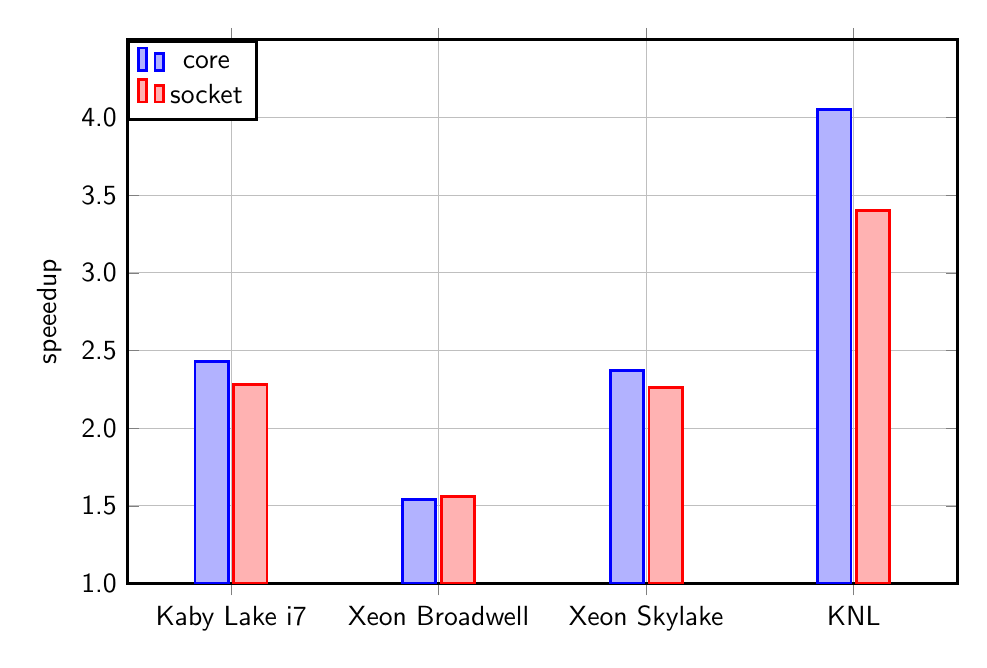
\begin{tikzpicture}
       \begin{axis}[
            ylabel=speeedup,
            ybar,
            height=0.7\textwidth,
            width=\textwidth,
            xmin=50, xmax=450,
            ymin=1, ymax=4.5,
            ytick={1.0, 1.5, 2.0, 2.5, 3.0, 3.5, 4.0},
            yticklabels={1.0, 1.5, 2.0, 2.5, 3.0, 3.5, 4.0},
            xtick={100,200,300,400},
            xticklabels={Kaby Lake i7, Xeon Broadwell, Xeon Skylake, KNL},
            line width=1pt,
            %ylabel style={yshift=-0pt},
            %yticklabel style={xshift=-2pt},
            legend style = {at={(0,1)}, anchor=north west},
            grid=major,
            %tick label style={rotate=20},
            bar width=12pt]
           % single core
           \addplot coordinates {
                    (100,2.43) (200,1.54) (300,2.37) (400,4.05)};
           % node/socket
           \addplot coordinates {
                    (100,2.28) (200,1.56) (300,2.26) (400,3.40)};

           \legend{core, socket}
       \end{axis}
    \end{tikzpicture}


%\begin{tikzpicture}
%    \begin{axis}[
%        ylabel=speeedup,
%        ybar,
%        width=0.5\textwidth,
%        height=0.3\textwidth,
%        xmin=50, xmax=450,
%        ymin=1, ymax=4.5,
%        ytick={1.0, 1.5, 2.0, 2.5, 3.0, 3.5, 4.0},
%        xtick={100,200,300,400},
%        xticklabels={i7 Laptop, Xeon Broadwell, Xeon Skylake, KNL},
%        ylabel style={yshift=-10pt},
%        yticklabel style={xshift=-2pt},
%        legend style = {at={(0,1)}, anchor=north west},
%        grid=major,
%        tick label style={rotate=20},
%        bar width=12pt]
%       % single core
%       \addplot coordinates {
%                (100,2.43) (200,1.54) (300,2.37) (400,4.05)};
%       % node/socket
%       \addplot coordinates {
%                (100,2.28) (200,1.56) (300,2.26) (400,3.40)};
%
%       \legend{core, socket}
%   \end{axis}
%\end{tikzpicture}

\end{document}

